\documentclass[../../main/main.tex]{subfiles}
\graphicspath{{./figures/}}
\usepackage{custikz}

\dominitoc
\faketableofcontents

\renewcommand{\mtcSfont}{\small\bfseries}
\renewcommand{\mtcSSfont}{\footnotesize}
\mtcsettitle{minitoc}{}
\mtcsetrules{*}{off}

\makeatletter
\renewcommand{\@chapapp}{Thermodynamique -- chapitre}
\makeatother

% \toggletrue{student}
% \toggletrue{corrige}
% \renewcommand{\mycol}{black}
% \renewcommand{\mycol}{gray}

\hfuzz=5.003pt

\begin{document}
\setcounter{chapter}{3}

% \settype{book}
% \settype{prof}
% \settype{stud}

\chapter{Second principe et machines thermiques}

\vspace*{\fill}

\begin{tcn}*(appl)<ctc>{\iconsomm~Sommaire}
	\let\item\olditem
	\vspace{-15pt}
	\minitoc
	\vspace{-25pt}
\end{tcn}

\begin{tcn}*[sidebyside, sidebyside align=top,
		fontupper=\small, fontlower=\small](appl)<ctb>"how"'t'{Capacités exigibles}
	\begin{itemize}[label=\rcheck]
		\item Interpréter qualitativement l'entropie en termes de désordre
		      statistique à l'aide de la formule de Boltzmann fournie.

		\item Définir un système fermé et établir pour ce système un bilan
		      entropique.

		\item Relier la création d'entropie à une ou plusieurs causes physiques de
		      l'irréversibilité.

		\item Analyser le cas particulier d'un système en évolution adiabatique.

		\item Utiliser l'expression fournie de la fonction d'état entropie.

		\item Exploiter l'extensivité de l'entropie.
	\end{itemize}
	\tcblower
	\begin{itemize}[label=\rcheck]
		\item Citer et utiliser la loi de Laplace et ses conditions
		      d'application.

		\item Donner le sens des échanges énergétiques pour un moteur ou un
		      récepteur thermique ditherme.

		\item Analyser un dispositif concret et le modéliser par une machine
		      cyclique ditherme.

		\item Définir un rendement ou une efficacité et les relier aux énergies
		      échangées au cours d'un cycle.

		\item Justifier et utiliser le théorème de Carnot.

		\item Citer quelques ordres de grandeur des rendements des machines
		      thermiques réelles actuelles.

		\item Expliquer le principe de la cogénération.
	\end{itemize}
\end{tcn}

\vspace*{\fill}

\newpage

\vspace*{\fill}
% {
% \begin{boxes}
\begin{tcn}[sidebyside, fontupper=\small, fontlower=\small](appl)<ctb>"check"'t'{L'essentiel}
	\begin{tcn}(defi)<ctc>'t'{Définitions}
		\tcblistof[\paragraph*]{defi}{\hspace*{4.8pt}}
	\end{tcn}
	% \begin{tcn}(rapp)<ctc>'t'{Rappels}
	% 	\tcblistof[\paragraph*]{rapp}{\hspace*{4.8pt}}
	% \end{tcn}
	\begin{tcn}(prop)<ctc>'t'{Propriétés}
		\tcblistof[\paragraph*]{prop}{\hspace*{4.8pt}}
		\tcblistof[\paragraph*]{loi}{\hspace*{4.8pt}}
		% \tcblistof[\paragraph*]{theo}{\hspace*{4.8pt}}
	\end{tcn}
	% \begin{tcn}(coro)<ctc>'t'{Corollaires}
	%   \tcblistof[\paragraph*]{coro}{\hspace*{4.8pt}}
	% \end{tcn}
	\begin{tcn}(demo)<ctc>'t'{Démonstrations}
		\tcblistof[\paragraph*]{demo}{\hspace*{4.8pt}}
		\tcblistof[\paragraph*]{prev}{\hspace*{4.8pt}}
	\end{tcn}
	% \begin{tcn}(inte)<ctc>'t'{Interprétations}
	%   \tcblistof[\paragraph*]{inte}{\hspace*{4.8pt}}
	% \end{tcn}
	% \begin{tcn}(tool)<ctc>'t'{Outils}
	% 	\tcblistof[\paragraph*]{tool}{\hspace*{4.8pt}}
	% \end{tcn}
	% \begin{tcn}(nota)<ctc>'t'{Notations}
	%   \tcblistof[\paragraph*]{nota}{\hspace*{4.8pt}}
	% \end{tcn}
	% \begin{tcn}(appl)<ctc>'t'{Applications}
	%   \tcblistof[\paragraph*]{appl}{\hspace*{4.8pt}}
	% \end{tcn}
	% \begin{tcn}(rema)<ctc>'t'{Remarques}
	%   \tcblistof[\paragraph*]{rema}{\hspace*{4.8pt}}
	% \end{tcn}
	% \begin{tcn}(exem)<ctc>'t'{Exemples}
	%   \tcblistof[\paragraph*]{exem}{\hspace*{4.8pt}}
	% \end{tcn}
	% \begin{tcn}*(ror)<ctc>"hart"'t'{Points importants}
	%   \tcblistof[\paragraph*]{ror}{\hspace*{4.8pt}}
	% \end{tcn}
	% \begin{tcn}(impo)<ctc>'t'{Erreurs communes}
	%   \tcblistof[\paragraph*]{impo}{\hspace*{4.8pt}}
	% \end{tcn}
	\tcblower
	% \begin{tcn}(defi)<ctc>'t'{Définitions}
	%   \tcblistof[\paragraph*]{defi}{\hspace*{4.8pt}}
	% \end{tcn}
	% \begin{tcn}(rapp)<ctc>'t'{Rappels}
	%   \tcblistof[\paragraph*]{rapp}{\hspace*{4.8pt}}
	% \end{tcn}
	% \begin{tcn}(prop)<ctc>'t'{Propriétés}
	%   \tcblistof[\paragraph*]{prop}{\hspace*{4.8pt}}
	%   \tcblistof[\paragraph*]{loi}{\hspace*{4.8pt}}
	%   \tcblistof[\paragraph*]{theo}{\hspace*{4.8pt}}
	% \end{tcn}
	% \begin{tcn}(coro)<ctc>'t'{Corollaires}
	%   \tcblistof[\paragraph*]{coro}{\hspace*{4.8pt}}
	% \end{tcn}
	% \begin{tcn}(demo)<ctc>'t'{Démonstrations}
	% 	\tcblistof[\paragraph*]{demo}{\hspace*{4.8pt}}
	% 	\tcblistof[\paragraph*]{prev}{\hspace*{4.8pt}}
	% \end{tcn}
	\begin{tcn}(inte)<ctc>'t'{Interprétations}
		\tcblistof[\paragraph*]{inte}{\hspace*{4.8pt}}
	\end{tcn}
	\begin{tcn}(inte)<ctc>'t'{Implications}
		\tcblistof[\paragraph*]{impl}{\hspace*{4.8pt}}
	\end{tcn}
	% \begin{tcn}(tool)<ctc>'t'{Outils}
	%   \tcblistof[\paragraph*]{tool}{\hspace*{4.8pt}}
	% \end{tcn}
	% \begin{tcn}(nota)<ctc>'t'{Notations}
	%   \tcblistof[\paragraph*]{nota}{\hspace*{4.8pt}}
	% \end{tcn}
	\begin{tcn}(appl)<ctc>'t'{Applications}
		\tcblistof[\paragraph*]{appl}{\hspace*{4.8pt}}
	\end{tcn}
	% \begin{tcn}(rema)<ctc>'t'{Remarques}
	%   \tcblistof[\paragraph*]{rema}{\hspace*{4.8pt}}
	% \end{tcn}
	% \begin{tcn}(exem)<ctc>'t'{Exemples}
	% 	\tcblistof[\paragraph*]{exem}{\hspace*{4.8pt}}
	% \end{tcn}
	\begin{tcn}*(ror)<ctc>"hart"'t'{Points importants}
		\tcblistof[\paragraph*]{ror}{\hspace*{4.8pt}}
	\end{tcn}
	\begin{tcn}(impo)<ctc>'t'{Erreurs communes}
		\tcblistof[\paragraph*]{impo}{\hspace*{4.8pt}}
	\end{tcn}
\end{tcn}
% \end{boxes}
% }%

\vspace*{\fill}
\newpage

\section{L'entropie}

Le premier principe traduit la conservation de l'énergie lors de l'évolution
d'un système. Cependant il ne dit rien sur le sens de cette évolution~: peut–on
retourner de l'état final à l'état initial en passant par le même chemin, ou
faut–il appliquer des contraintes drastiquement différentes~?

La réponse est non~: un système isolé ne peut subir n'importe quelle
transformation ! Un système évoluera toujours d'un état hors équilibre vers un
état d'équilibre, et pas l'inverse.

Ce constat est \textit{a priori} intuitif, puisqu'il décrit l'évolution même du
temps et notre expérience de son écoulement (un verre cassé ne se répare pas
tout seul), mais il est nécessaire de l'introduire mathématiquement.

\subsection{Statistique}
Pour comprendre la notion d'entropie, on doit s'intéresser à la probabilité
qu'un événement physique survienne.

Reprenons l'exemple de la détente de \textsc{Joule Gay-Lussac}\ftn{Pour une
	visualisation animée, voir la simulation de la diffusion de PhET Colorado~:
	\url{https://phet.colorado.edu/sims/html/diffusion/latest/diffusion_all.html}}~:
soit $N$ molécules de gaz confinées dans une enceinte indéformable et athermane
de volume total $V$, séparée en deux volumes égaux par une cloison. Dans l'état
initial, on injecte toutes les particules dans le compartiment de gauche.

\begin{figure}[htbp!]
	\sswitch{
		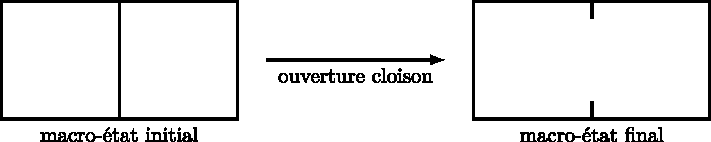
\includegraphics[scale=1]{jgl_intro-stud}
	}{
		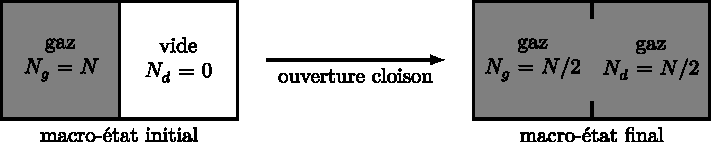
\includegraphics[scale=1]{jgl_intro}
	}
	\caption{Évolution spontanée dans l'expérience de \textsc{Joule Gay-Lussac}}
\end{figure}

On définit les éléments suivants~:
\begin{tcb}(defi){États statistiques d'un système}
	\begin{itemize}
		\item[b]{Micro-état}: \psw{c'est la donnée de l'état de \textbf{chaque}
			particule (vitesse, position)~;}
		\item[b]{Macro-état}: \psw{c'est la donnée des \textbf{grandeurs
				macroscopiques} (pression, température…)}
		\item[b]{Nombre de configurations}: noté $\Omega$, \psw{c'est le nombre de
			\textbf{micro-états compatibles avec un macro-état}.}
	\end{itemize}
\end{tcb}

On s'intéresse alors au nombre de particules dans le compartiment de gauche
$N_g$ et dans le compartiment de droite $N_d$~: ce sont des macro-états, qui
peuvent être réalisés par différents micro-états. Par exemple, pour $N = 2$, il
y a $\Omega\ind{tot} = 4$ micro-états différents, et pour le macro-état $N_g$ il
y en a 3 différents~:

\begin{figure}[htbp!]
	\sswitch{
		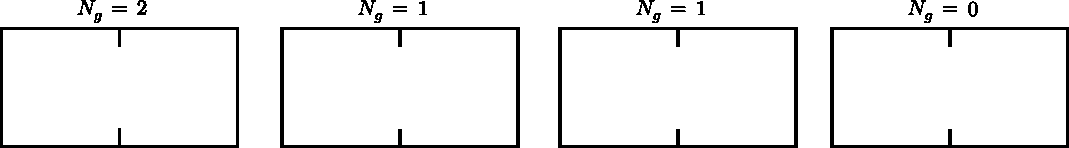
\includegraphics[width=\linewidth]{jgl_n2-stud}
	}{
		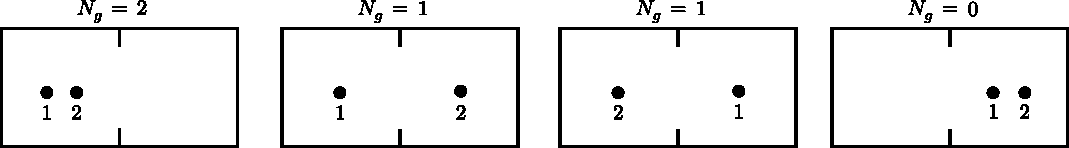
\includegraphics[width=\linewidth]{jgl_n2}
	}
	\vspace{-15pt}
	\caption{Décompte des micro-états pour 2 particules}
\end{figure}

\textbf{Chacun de ces états est possiblement accessible}, mais il apparaît
clairement que l'un d'entre eux est plus \textbf{probable} que les autres~: il y
a deux manières d'arranger les particules pour avoir le macro-état $N_g = 1$,
contre une seule pour les deux autres. On peut remplir le tableau suivant~:

\begin{center}
	\begin{tabular}{ccc}
		\toprule
		\textbf{Macro-état}     &
		\textbf{Configurations} &
		\textbf{Probabilité}
		\\
		\midrule
		$N_g = 0$               &
		\psw{$\Omega = 1$}      &
		$P(N_g = 0) = \psw{\DS\frac{\Omega}{\Omega\ind{tot}} = \num{0.25}}$
		\\
		$N_g = 1$               &
		\psw{$\Omega = 2$}      &
		$P(N_g = 1) = \psw{\DS\frac{\Omega}{\Omega\ind{tot}} = \num{0.50}}$
		\\
		$N_g = 2$               &
		\psw{$\Omega = 1$}      &
		$P(N_g = 2) = \psw{\DS\frac{\Omega}{\Omega\ind{tot}} = \num{0.25}}$
		\\
		\bottomrule
	\end{tabular}
\end{center}

On voit alors apparaître la notion d'entropie et également ce qui définit la
flèche du temps~: les états évoluent vers les \textbf{macro-états les plus
	probables}, c'est-à-dire ceux \textbf{de plus grandes configurations}.

\noindent
\begin{minipage}[c]{.50\linewidth}
	Pour appliquer cette idée à la thermodynamique, il faut l'appliquer à des
	systèmes thermodynamiques, c'est-à-dire comprenant un grand nombre de
	particules. Dans ce cas, $\Omega(N_g)$ se calcule avec\ftn{On retrouve ce
		calcul derrière le triangle de \textsc{Pascal} en mathématiques.}~:
	\[
		\Omega(N_g) = \psw{\mqty(N_g\\N) = \frac{N_g!}{N_g!(N-N_g)!}}
	\]
\end{minipage}
\hfill
\begin{minipage}[c]{.48\linewidth}
	\begin{center}
		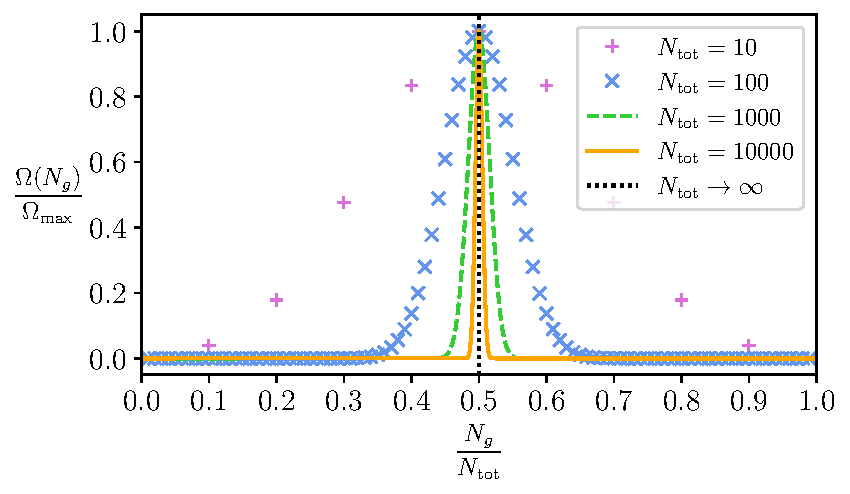
\includegraphics[width=\linewidth]{proba_etat}
	\end{center}
\end{minipage}

Cette distribution est alors \textbf{maximale pour $N_g = N/2$}, c'est-à-dire
$\Omega\ind{max} = \Omega(N/2)$, mais surtout \textbf{décroît exponentiellement
	vite pour $N_g \neq N/2$}.

\begin{tcb*}(prop){Formule de \textsc{Boltzmann}}
	L'entropie d'un système thermodynamique \textbf{isolé} et \textbf{à
		l'équilibre} est une fonction d'état extensive, donnée par la formule
	\smallbreak
	\begin{isd}
		\psw{%
			\[
				\boxed{S = k_B \ln \Omega}
			\]
		}%
		\vspace{-15pt}
		\tcblower
		\tcbsubtitle{\fatbox{\textbf{Unité}}}
		\psw{%
			\[
				\si{J.K^{-1}}
			\]
		}%
		\vspace{-15pt}
	\end{isd}
	avec $k_B = \SI{1.38e-23}{J.K^{-1}}$ la constante de \textsc{Boltzmann} et
	$\Omega$ le nombre de configurations décrivant le macro-état observé.
\end{tcb*}
\begin{tcb*}(inte){Entropie selon \textsc{Boltzmann}}
	Ainsi, plus $\Omega$ est grand, plus l'entropie est grande~: l'entropie est
	une mesure de la \textbf{probabilité de réalisation} d'un macro-état. Étant
	donné que les états les moins probables sont les plus «~ordonnés~» ($\Omega =
		1$), on dit également que \textbf{l'entropie est une mesure du désordre
		microscopique} d'un système.
	\bigbreak
	Elle \textbf{évolue naturellement vers son augmentation}, et mène à de
	l'irréversibilité~: par un phénomène statistique collectif propre aux systèmes
	de grand nombre de particule, l'évolution vers des états ordonnés est
	\textbf{statistiquement impossible}.
\end{tcb*}

C'est cette idée qui régit l'évolution du gaz de l'état initial à l'état final
dans l'expérience de \textsc{Joule Gaz-Lussac}, mais qui régit également
l'équilibre des températures de deux gaz de températures initialement
différentes. Voir l'animation précédente pour la simulation.

\begin{tcb}(exem)<lftt>{Entropie d'une goutte d'encre}
	En plaçant une goutte de colorant dans de l'eau, celle-ci se répartit dans
	l'espace disponible, \textbf{sans retour en arrière possible}, ce qui
	s'explique pas les micro-états compatibles avec chaque situation.
	\begin{center}
		\begin{tabularx}{.7\linewidth}{|l|Y|Y|}
			\hline
			                                                &
			\textbf{État initial}                           &
			\textbf{État ultérieur}
			\\\hline
			\rotatebox[origin=c]{90}{Macro-état}            &
			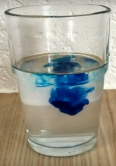
\includegraphics[height=3cm,
			margin=0pt 1ex 0pt 1ex, valign=m]{encre_1}      &
			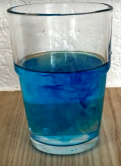
\includegraphics[height=3cm, valign=m]{encre_2}
			\\\hline
			\rotatebox[origin=c]{90}{Micro-état}            &
			
\includegraphics[height=3cm,
			margin=0pt 1ex 0pt 1ex, valign=m]{encre_1_etat} &
			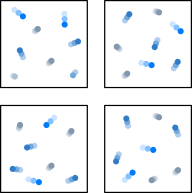
\includegraphics[height=3cm, valign=m]{encre_2_etat}
			\\\hline
		\end{tabularx}
	\end{center}
\end{tcb}

\subsection{Irréversibilité}
D'après la section précédente, l'entropie évolue naturellement dans le sens de
son augmentation. C'est pourquoi la mise en contact d'un bloc de cuivre chaud
dans de l'eau donne l'évolution temporelle suivante~:
\begin{figure}[htbp]
	\centering
	\sswitch{
		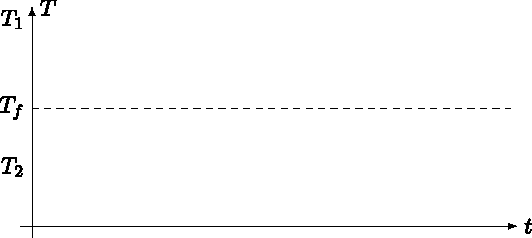
\includegraphics[scale=1]{evol_temp-stud}
	}{
		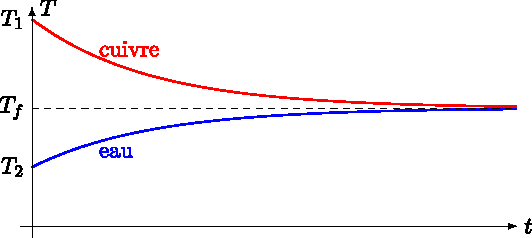
\includegraphics[scale=1]{evol_temp}
	}
\end{figure}

D'une manière générale, deux corps de températures différentes en contact
équilibrent leurs températures~:

\begin{figure}[htbp]
	\centering
	\sswitch{
		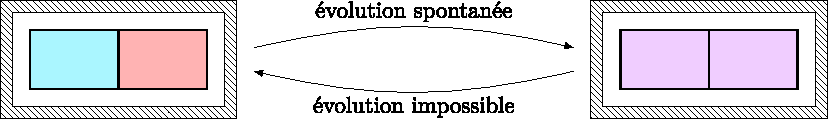
\includegraphics[scale=1]{evol_temp_gen-stud}
	}{
		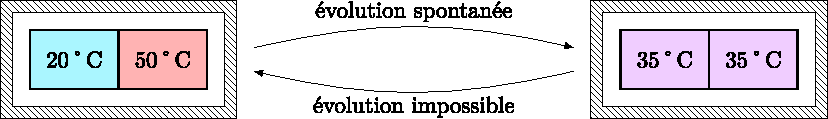
\includegraphics[scale=1]{evol_temp_gen}
	}
\end{figure}

On observe la même chose en mécanique~:

\begin{figure}[htbp]
	\centering
	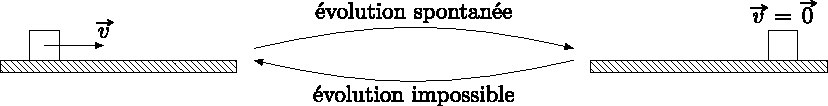
\includegraphics[scale=1]{evol_vits}
\end{figure}

On a alors les critères suivants~:
\begin{tcb*}(prop){Transformations réversibles ou non}
	\begin{itemize}
		\item[b]{Réversible}: une transformation est réversible si~:
		\begin{itemize}
			\item \psw{elle est quasi-statique, c'est-à-dire en équilibre interne à
				      tout instant~;}
			\item \psw{on peut inverser le sens d'évolution par une modification
				      infinitésimale des paramètres extérieurs}
		\end{itemize}
		\item[b]{Irréversible}: le système ne peut \textbf{pas suivre} la
		transformation en \textbf{sens inverse} en passant par les mêmes états
		intermédiaires.
	\end{itemize}
	Les causes de l'irréversibilité sont donc toute inhomogénéité interne
	(température, pression), tous les frottements (transfert d'énergie sous forme
	de chaleur), et les réactions chimiques.
\end{tcb*}

\subsection{Second principe de la thermodynamique}
\begin{tcb*}(prop){Second principe de la thermodynamique}
	Il existe une \textbf{fonction d'état}, nommée \textbf{entropie} et notée $S$,
	qui est \textbf{extensive} mais qui \textbf{ne se conserve pas}. Au cours
	d'une transformation d'un système fermé, elle varie selon la loi~:
	\psw{%
		\[
			\boxed{\Delta{S} = S\ind{ech} + S\ind{créée}}
			\Lra
			\boxed{\delta{S} = \delta{S}\ind{ech} + \delta{S}\ind{créée}}
		\]
	}%
	\begin{isd}
		\tcbsubtitle{\fatbox{\textbf{Entropie échangée}}}
		Pour un système en contact avec un thermostat, l'entropie échangée est
		\psw{%
			\[
				S\ind{ech} = \frac{Q}{T\ind{cst}}
				\Lra
				\delta{S}\ind{ech} = \frac{\delta{Q}}{T\ind{cst}}
			\]
		}%
		et elles se somment pour un contact avec plusieurs thermostats.
		\tcblower
		\tcbsubtitle{\fatbox{\textbf{Entropie créée}}}
		L'entropie créée ne \textbf{peut qu'augmenter}, et on a donc~:
		\smallbreak
		\noindent
		\begin{minipage}[c]{.60\linewidth}
			$\left.
				\parbox{1\linewidth}{%
					\begin{itemize}
						\item[b]{Irréversible}: $\psw{S_c > 0}$
						\item[b]{Réversible}: $\psw{S_c = 0}$
					\end{itemize}
				}
				\right\}$
		\end{minipage}
		\hfill
		\begin{minipage}[c]{.35\linewidth}
			\hspace{20pt}
			\psw{$S_c \geq 0$}
		\end{minipage}
	\end{isd}
\end{tcb*}

\begin{center}
	\begin{tikzpicture}
		\draw (0,0) rectangle (4,2);
		\draw (2,1) node{fluide};

		\draw (-3.5,1) circle (1);
		\draw (-3.5,1) node[text centered,text width=2.5cm]{Source \\ froide \\ $T_f$};


		\draw (7.5,1) circle (1);
		\draw (7.5,1) node[text centered,text width=2.5cm]{Source \\ chaude \\ $T_c$};

		\draw[simplef] (-2.5,1)--(0,1)node[midway,above]{$Q_f$};
		\draw[simplef] (6.5,1)--(4,1)node[midway,above]{$Q_c$};
		\draw[simplef] (2,-1)--(2,0)node[midway,right]{$W$};

		\draw [red,->,>=latex,very thick] (-2,0.75)--(-1,0.75);
		\draw [red,->,>=latex,very thick] (5,0.75)--(6,0.75);
		\draw [red,->,>=latex,very thick] (1.75,-0.95)--(1.75,-0.25);

	\end{tikzpicture}
\end{center}

\end{document}

% \begin{center}
% 	\begin{tikzpicture}[scale=1.3]
% 		\draw [->](0,0) -- (0,3.5) node[anchor=west]{$P$};
% 		\draw [->](0,0) -- (5.5,0) node[anchor=west]{$V$};
%
% 		\draw[dashed] plot [domain=0.8:5] (\x,3/\x) node[below]{$T_f$};
% 		\draw[very thick, red,simplef] plot [domain=1.5:3] (\x,3/\x);
% 		\draw[very thick, red,simplef] plot [domain=1.0203:1.5] (\x,{3.5282/(\x^(1.4))});
% 		\draw[dashed] plot [domain=0.8:5] (\x,3.5/\x) node[above]{$T_c$};
% 		\draw[very thick, red,simplef] plot [domain=2.0406:1.0203] (\x,3.5/\x);
% 		\draw[very thick, red,simplef] plot [domain=3:2.0406] (\x,{4.6555/(\x^(1.4))});
%
% 		\fill (3,1) circle(0.04);
% 		\fill (1.5,2) circle(0.04);
% 		\fill (1.0203,3.43) circle(0.04);
% 		\fill (2.0406,1.72) circle(0.04);
%
% 		\node[above] at (3,1) {A};
% 		\node[left] at (1.5,2) {D};
% 		\node[right] at (1.0203,3.43) {C};
% 		\node[right] at (2.0406,1.72) {B};
% 	\end{tikzpicture}
% \end{center}
